\section{Utilization at Interconnection Points}\label{sec:findings}

In this section, we present preliminary analysis of the utilization
measurements from the interconnect groups from the participating
ISPs. We survey the capacity and utilization of each interconnect group
both overall and by region. From October 2015 through February 2016, 
aggregate interconnect capacity has been roughly 50\% utilized at peak,
and capacity has grown consistently by about 3\% monthly, or about 19\% over the
five-month period.
In the rest of
this section, we explore the utilization characteristics of these links.

\begin{figure}[t]
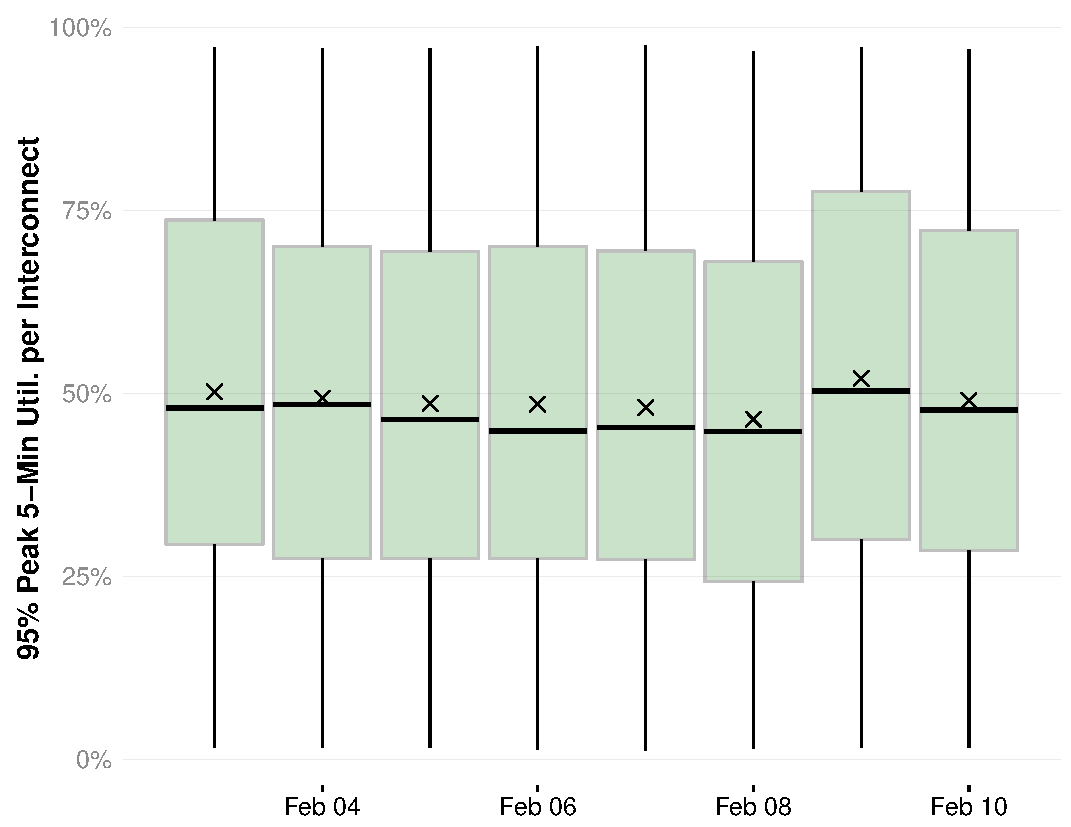
\includegraphics[width=\linewidth]{utilization-timeseries-box}
\caption{Utilization of each interconnect group over one week in
  February 2016, normalized by
  capacity of the interconnects.} 
\label{fig:utilization-timeseries}
\end{figure}


\begin{figure}[t]
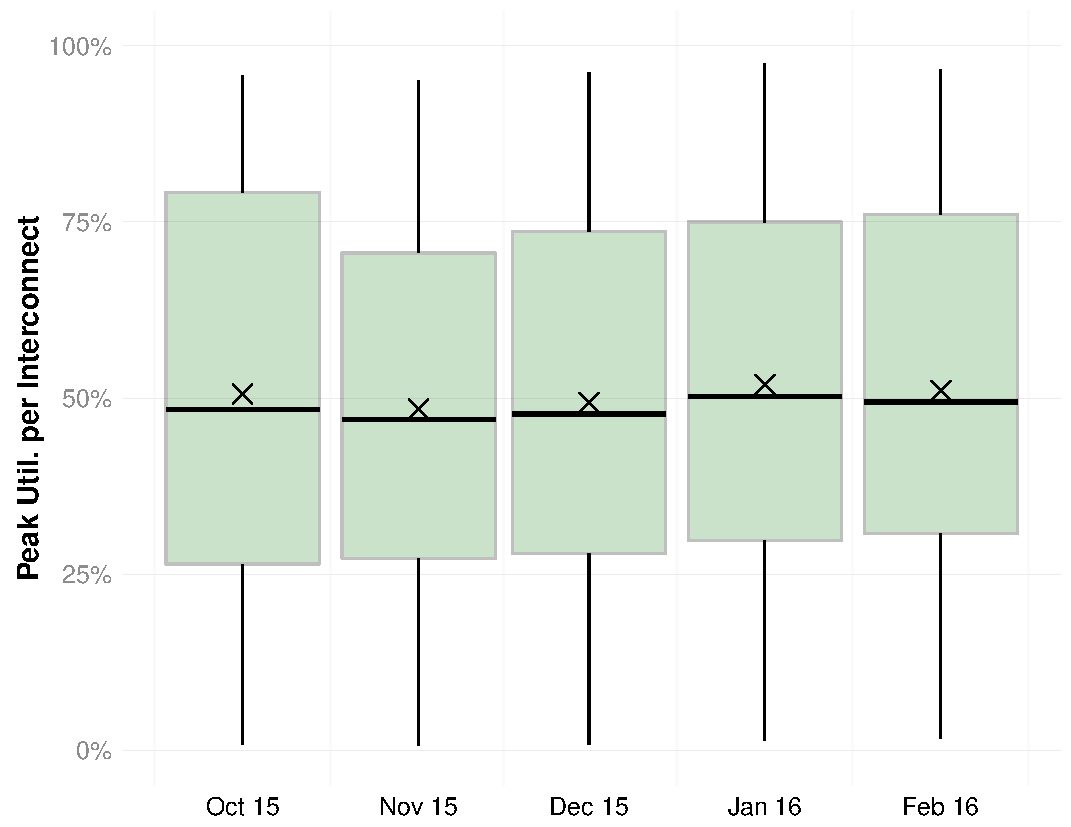
\includegraphics[width=\linewidth]{utilization-per-month-all-box}
\caption{Per-month utilization of all participating interconnects.} 
\label{fig:utilization-per-month-all}
\end{figure}



\begin{figure}[t]
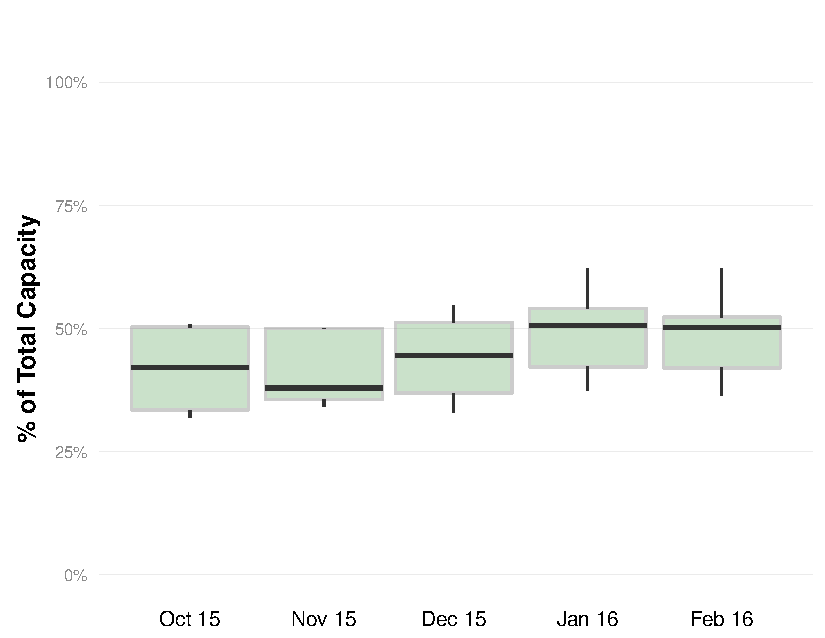
\includegraphics[width=\linewidth]{byISPdist}
\caption{Distribution of 95th percentile peak ingress utilization across
  all ISPs, with all ISPs equally weighted.} 
\label{fig:isp-dist}
\end{figure}


\begin{figure}[t!]
\begin{minipage}{1\linewidth}
\begin{subfigure}[b]{\linewidth}
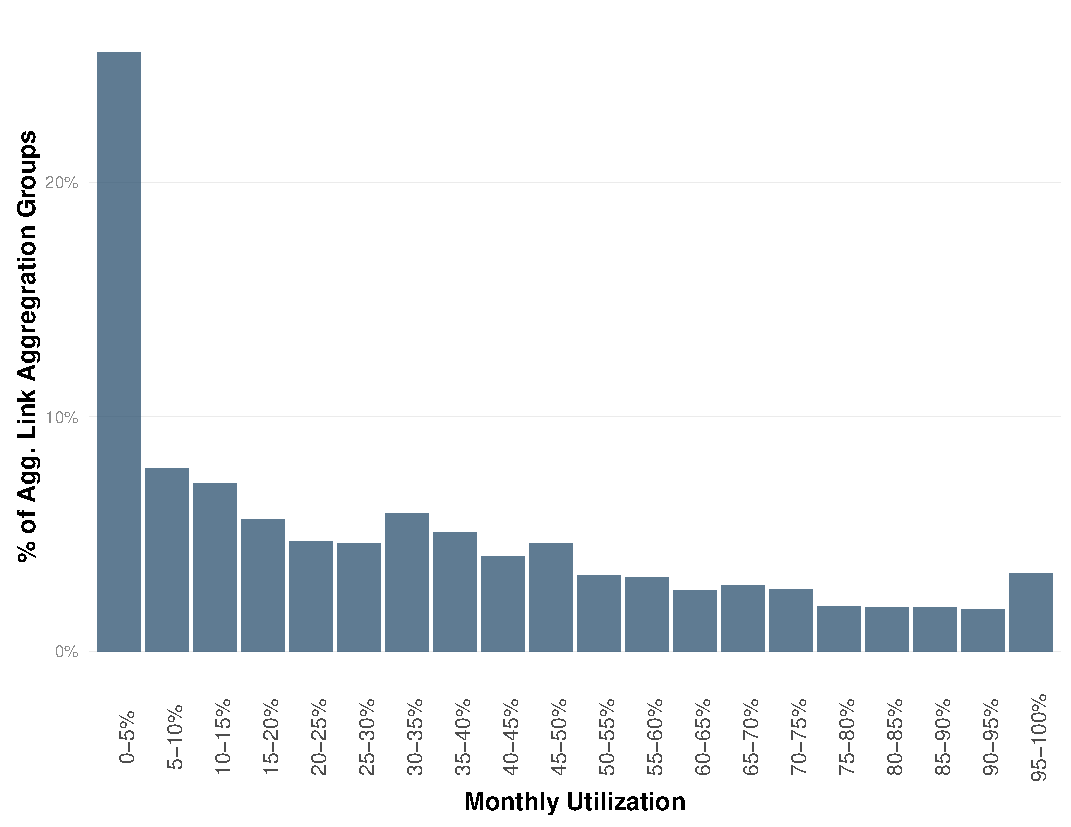
\includegraphics[width=\linewidth]{distribution-link-peak}
\caption{Weighted by links.\label{fig:dist-link-peak}}
\end{subfigure} \hfill
%
\begin{subfigure}[b]{\linewidth}
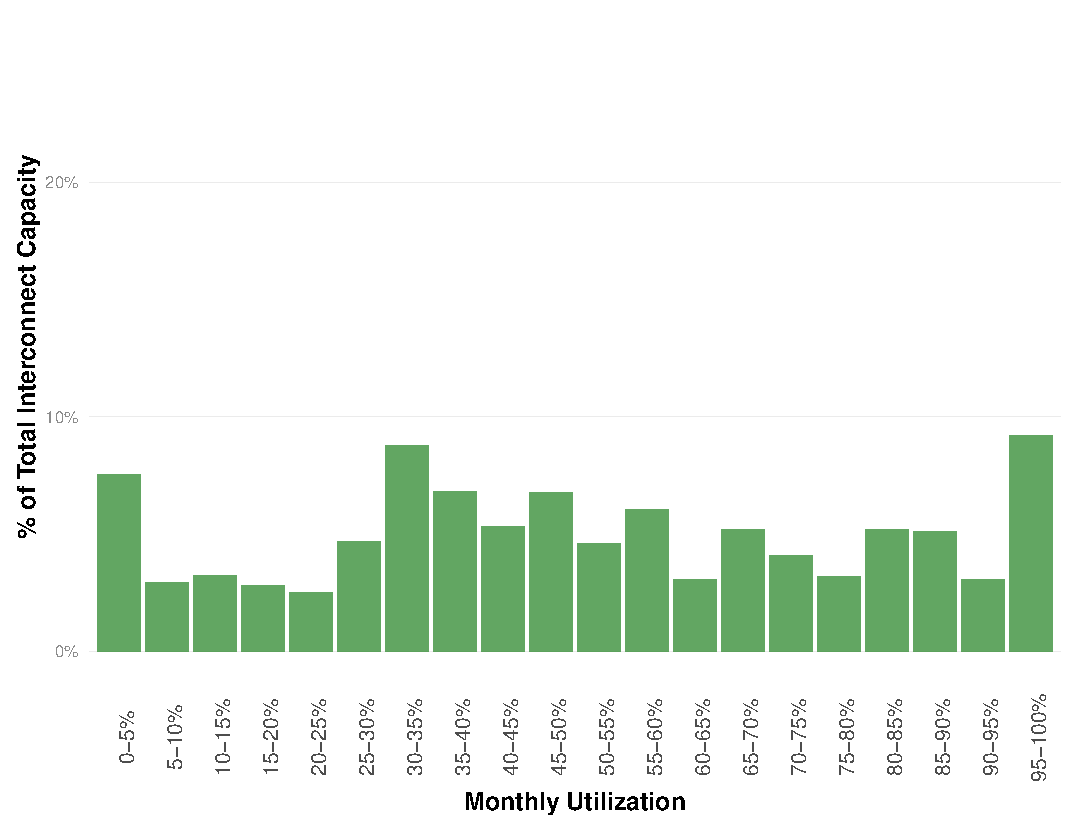
\includegraphics[width=\linewidth]{distribution-cap-peak}
\caption{Weighted by capacity.\label{fig:dist-cap-peak}}
\end{subfigure}
\end{minipage}
\caption{The fraction of interconnect capacity, weighted by the number
  of links and the amount of total capacity, respectively, whose 95th
  percentile utilization in a month experienced a particular utilization
  level. The figure shows statistics for February 2016.}
\label{fig:dist-peak}
\end{figure}

\begin{figure}[t]
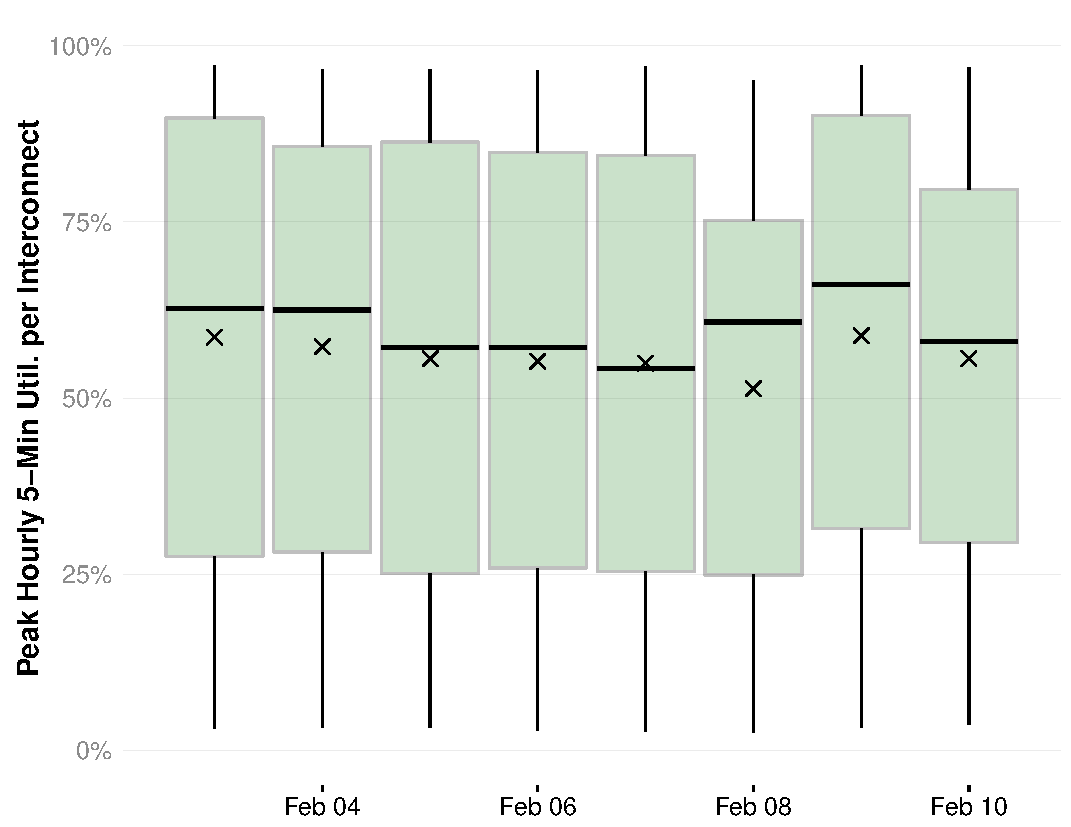
\includegraphics[width=\linewidth]{utilization-timeseries-box-chicago}
\caption{Utilization of each interconnect group over one week in
  February 2016 across
  interconnects in Chicago, IL, normalized by
  capacity of the interconnects.} 
\label{fig:utilization-timeseries-chicago}
\end{figure}


\begin{figure}[t!]
\begin{minipage}{1\linewidth}
\begin{subfigure}[b]{\linewidth}
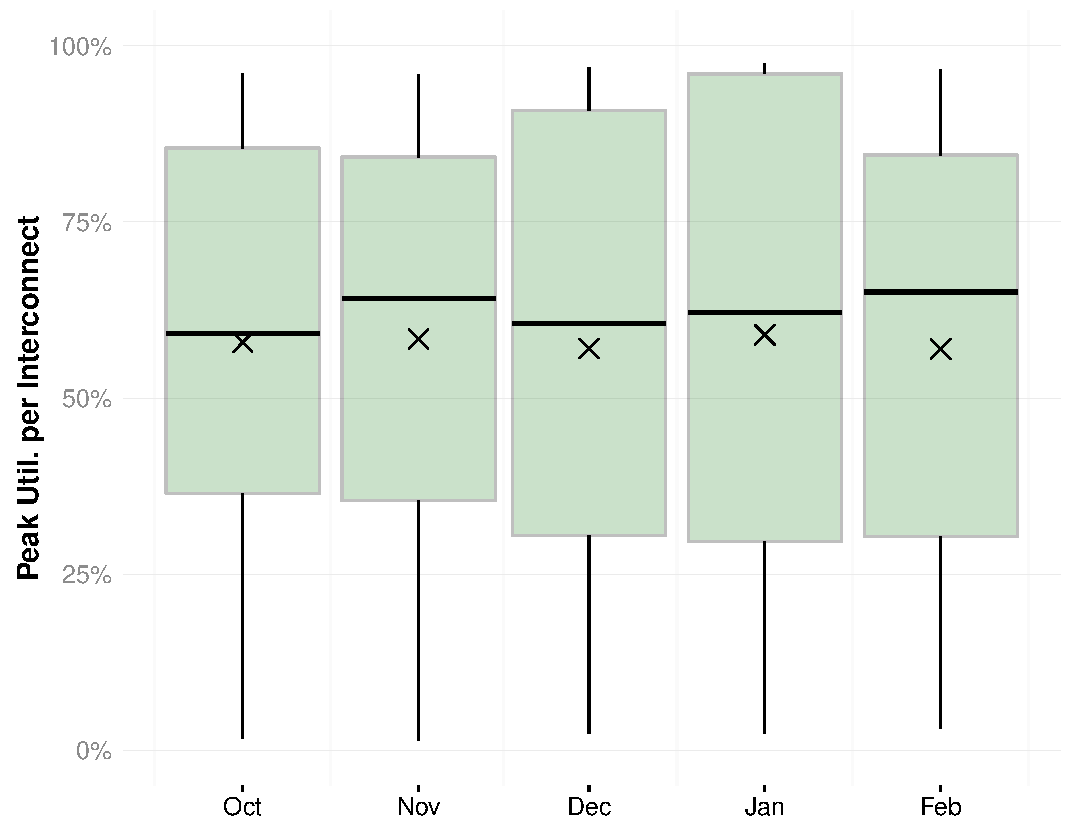
\includegraphics[width=\linewidth]{utilbox_graphs_2016-chicago}
\caption{Chicago.\label{fig:utilization-per-month-chicago}}
\end{subfigure} \hfill
%
\begin{subfigure}[b]{\linewidth}
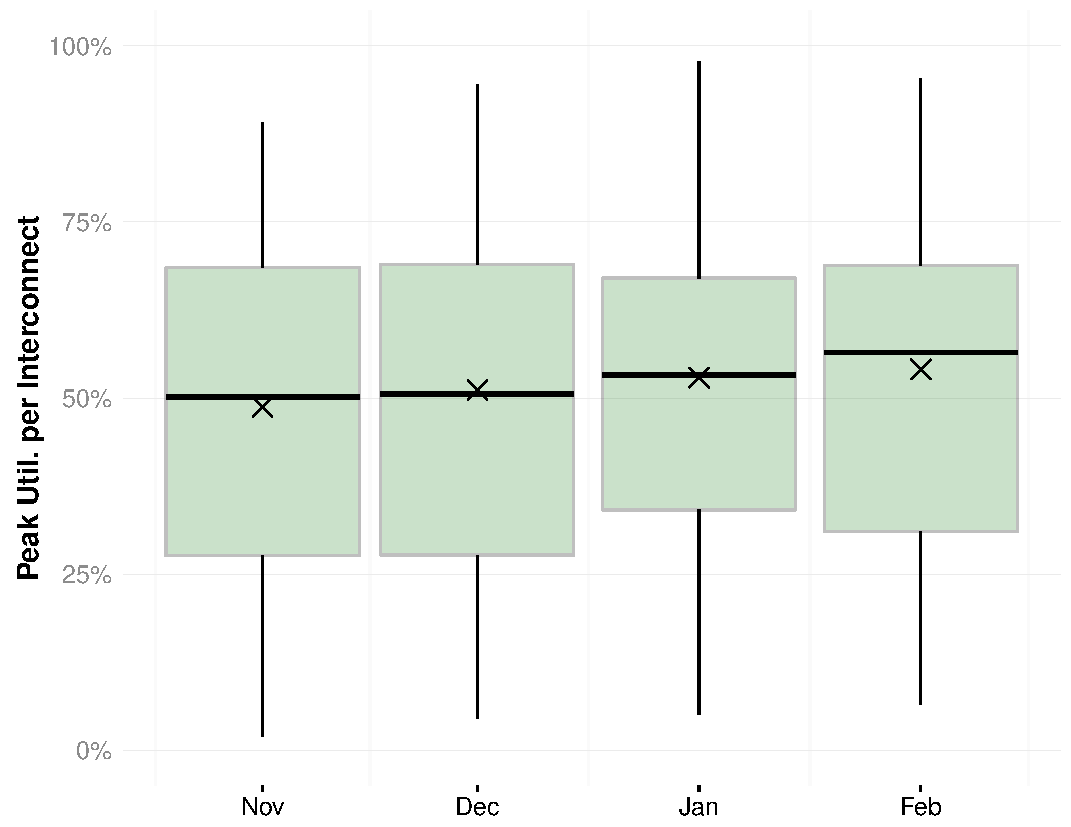
\includegraphics[width=\linewidth]{utilbox_graphs_2016-sanjose}
\caption{San Jose.\label{fig:utilization-per-month-sanjose}}
\end{subfigure}
\end{minipage}
\caption{Per-month utilization of participating interconnects in two
  example regions.}
\label{fig:utilization-per-month-compare}
\end{figure}

\subsection{Aggregate Utilization}

Figure~\ref{fig:utilization-timeseries} shows the
interconnect utilization over time, for a one-week period in
February 2016 across all regions. Each data point in the timeseries
shows a box plot illustrating the distribution of utilization
across interconnect points. The median utilization across interconnects
is consistently below 50\%, even at peak times, and many of the links
have significantly less utilization.  Less than 4\% of the link aggregation groups exceed 95\%
utilization in any five-minute interval, and the vast majority of the
link aggregation groups see much less utilization, even at peak
times. In the next section, we explore these trends for individual
regions. 

Recall that, due to aggregation, we cannot determine whether a
utilization of, say, 75\% indicates that there are no links in the
aggregation group running at full utilization. What we {\em can}
conclude, however, is that there {\em exist} links in the aggregation
group with sufficient spare capacity, and thus that most senders of
traffic have the ability to send traffic flows over links at the
interconnect that have spare capacity, even as other links may have high
utilization. 

% \xxx{Had we planned to show ISP
%   and jointly-sized separately? The plot is a bit small, so if we
%   separate this out into separate figures, it will be easier to
%   read. Additionally, why does one have green and the other not?  What
%   does that represent?}

Figure~\ref{fig:utilization-per-month-all} shows the distribution of
interconnect capacity by peak utilization over all five-minute intervals across link
aggregation groups for each month, for all aggregation groups. The box
plot shows the inter-quartile ranges, the horizontal line shows the
median utilization, and the whiskers show the 5th and 95th
percentiles. 

\subsection{Utilization by ISPs and Links}

Figure~\ref{fig:isp-dist} shows the distribution of 95th percentile peak ingress
utilization across all ISPs, normalized by capacity. The median ISP in
the group of seven ISPs experienced a 95th percentile peak ingress
utilization that was less typically around 50\% of the available
capacity.  This plot shows that each ISP has significant spare capacity
across its set of links and regions.  This figure does {\em not} indicate
whether a particular ISP is experiencing congestion in a particular
region, to a particular partner network, or across a set of links.

Unfortunately, we cannot show utilization for specific links or neighbor
networks, because the existence of a particular business relationship or
even the existence of a specific link in a region may reveal proprietary
information. We can, however, explore the utilization across the
aggregate of all links, which also shows the existence spare capacity.
Specifically, we can show how the characterization of peak utilization
across {\em all} links, weighted both by links and by overall capacity,
as shown in Figure~\ref{fig:dist-peak}.  Figure~\ref{fig:dist-link-peak}
shows the distribution of 95th percentile peak monthly utilization
across all links, for all participating ISPs.  This figure shows that
more than 25\% of all links are significantly underutilized, and that
less than 10\% of all links experience a 95th percentile peak
utilization that exceeds 90\%.  

In Figure~\ref{fig:dist-link-peak} all links are weighted equally, which
does not reveal whether there exists significant excess {\em capacity},
only whether there exist links that have spare capacity. Exploring
utilization where the set of links is weighted by their capacity reveals
more information. Figure~\ref{fig:dist-cap-peak} shows the same
distribution, where links are weighted by overall capacity. The figure
shows that links that account for about 10\% of overall interconnect
capacity experienced a 95th percentile peak utilization that exceeded
95\%.  Most of the capacity experienced significantly less utilization.

Together, these plots present a picture of the existence of spare
utilization across many of the interconnects that also account for much
of the capacity at interconnects. Certain answers remain obscured, such
as whether a particular partner network is experiencing persistent
congestion, or whether particular types of connections (e.g., paid
peering) are experiencing more or less congestion. Yet, the figures
above do reveal a general picture of (1)~all ISPs having spare capacity
in aggregate across interconnects; (2)~most interconnect capacity in
aggregate showing spare capacity at peak. Both of these conclusions
reveal significantly more than we have known to date; as this project
matures and we receive further feedback, we hope to make additional
views of the data available that also respect the private and
proprietary information of each ISP.

\subsection{Utilization by Region}

We also explored how utilization evolves over time in individual
regions, to determine whether utilization patterns at interconnects in
specific regions agreed with the overall general trends that we observed
in Figure~\ref{fig:utilization-timeseries}.
Figure~\ref{fig:utilization-timeseries-chicago} shows how utilization
evolves over time across interconnects in Chicago; the trends in this
specific region are similar to the overall trends.  The trends are
similar in other cities with busy interconnects; interconnects in
Atlanta show similar distributions.


Washington, New York, Dallas, and Los Angeles exhibit similar
utilization trends, although utilization exceeded 90\% less frequently
than it did in Chicago and Atlanta, the two busiest regions.
Figure~\ref{fig:utilization-per-month-compare} shows the distribution of
interconnect capacity across link aggregation groups over all
five-minute intervals. Figure~\ref{fig:utilization-per-month-chicago}
shows this distribution for a busier Interconnect (Chicago); 
Figure~\ref{fig:utilization-per-month-sanjose} shows the same
distribution for San Jose.
%
Interconnections in San Jose tend to have
lower median utilizations across link groups, although the highest loaded
link groups at peak time also follow similar trends as those that we
observed in Chicago.

%%%%%%%%%%%%%%%%%%%%%%%%%%%%%%%%%%%%%%%%%%%%%%%%%%%%%%%%%%%%

\if 0
\xxx{
Table~\ref{tab:interconnection-capacity} shows, for a representative
region, the 99th-percentile capacity for each ISP interconnection pair
for the month of January 2016 for both ISP, jointly, and partner-sized
interconnects. The table shows that, for the cases of ISP and
jointly-sized interconnect groups, there is spare capacity, even at peak
utilization. In the case of jointly-sized interconnects, the peak
utilization is considerably higher, in many regions. The table also
highlights that for a particular ISP and interconnect type, utilization
is relatively consistent across regions. 
}

\begin{figure}[t]
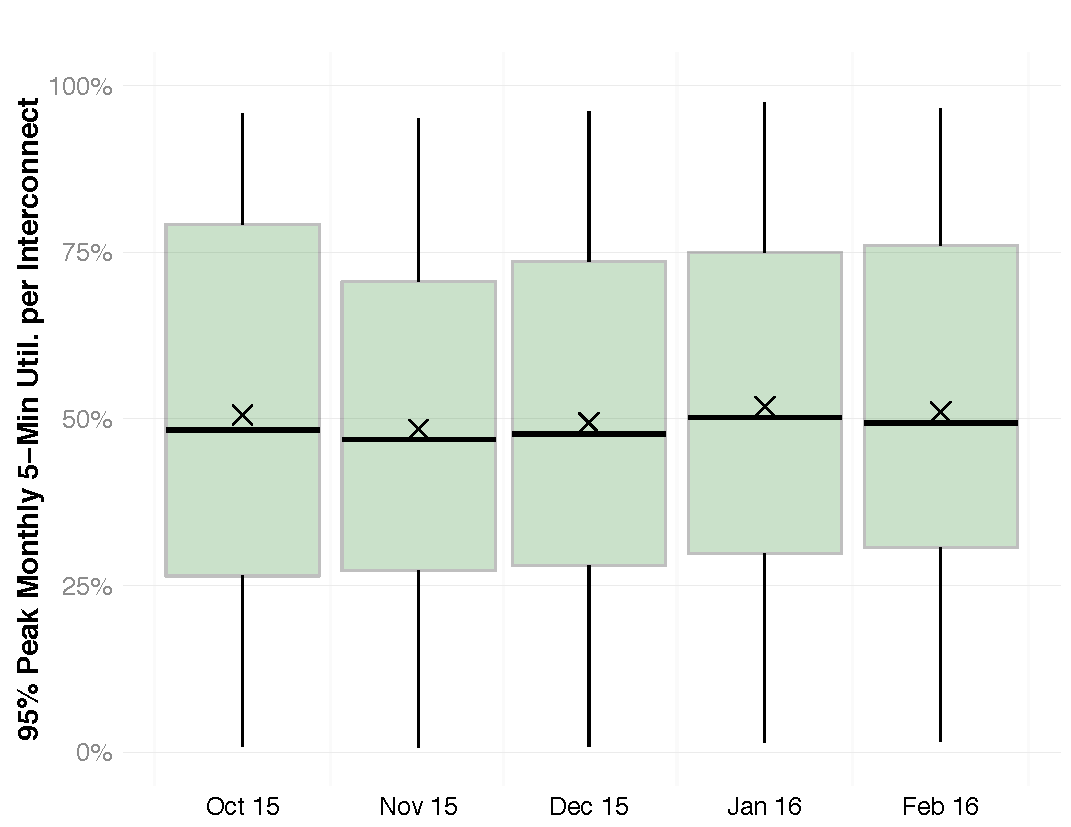
\includegraphics[width=\linewidth]{utilization-per-month-joint}
\caption{Per-month utilization of participating jointly-sized interconnects.} 
\label{fig:utilization-per-month-joint}
\end{figure}

\begin{figure}[t]
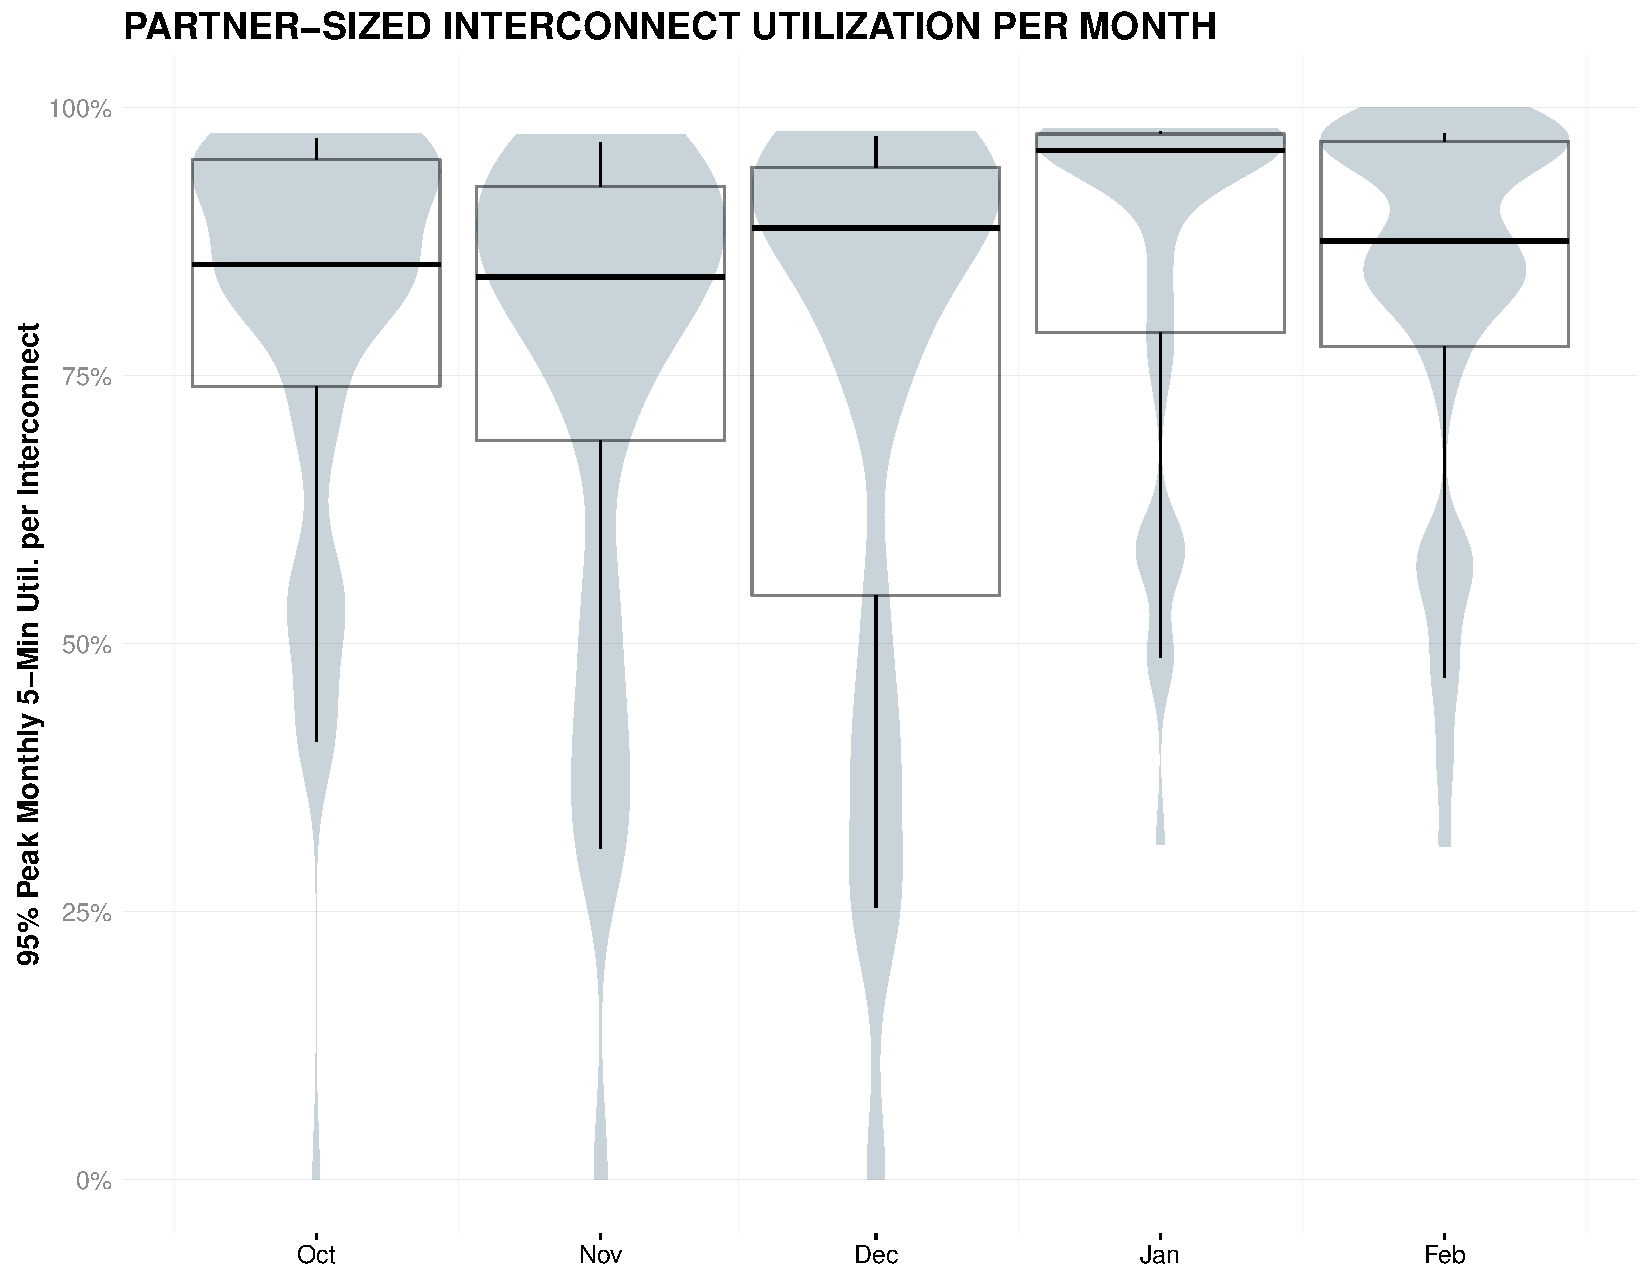
\includegraphics[width=\linewidth]{utilization-per-month-partner}
\caption{Per-month utilization of participating partner-sized interconnects.} 
\label{fig:utilization-per-month-partner}
\end{figure}


\fi
